\begin{figure}[H]
\centering
\begin{minipage}[t]{0.46\linewidth}
\raggedright\textbf{(a)}\par
\centering
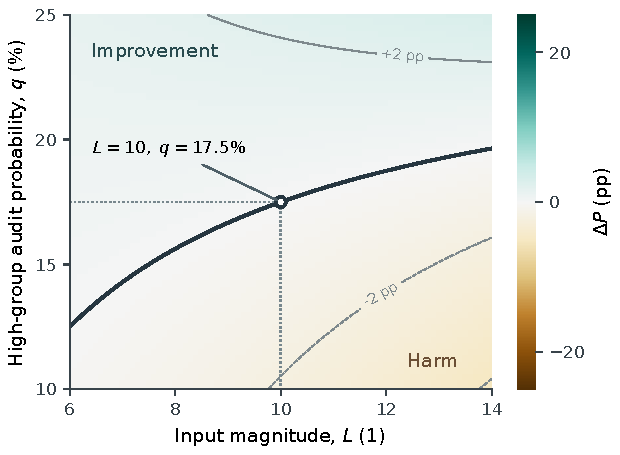
\includegraphics[width=\linewidth]{RSI-audit-figures-20261003/figures/final/audit_detail.pdf}
\end{minipage}\hfill
\begin{minipage}[t]{0.51\linewidth}
\raggedright\textbf{(b)}\par
\centering
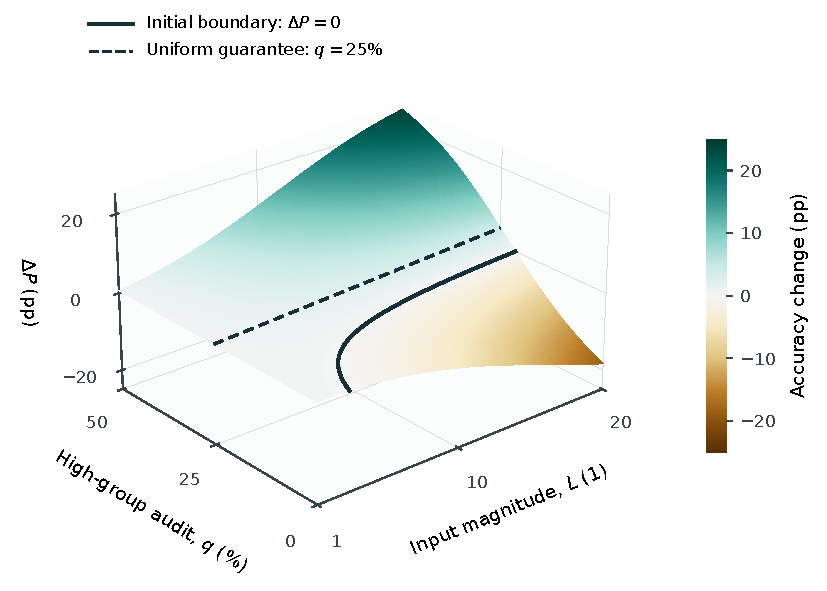
\includegraphics[width=\linewidth]{RSI-audit-figures-20261003/figures/final/audit_surface.pdf}
\end{minipage}
\caption{Supplementary views of the audited initial effect in
Figure~\ref{fig:population-overview}(c,d), with $a=0.75$, $b=0.5$,
$\theta_0=0$, and $\eta=0.1$.
(a) Refined boundary near $(L,q)=(10,0.175)$, using an independent refined grid.
(b) The same initial-effect response surface.
Both show $100[P(-\eta g_{S,q}(0))-1/2]$ in percentage points and retain
the $[-25,25]$ pp color scale. These are deterministic one-step
population calculations, not audited trajectories or language-model results.}
\label{fig:audit-supplement}
\end{figure}
